% ==============================================================================
% Copyright (C) 2017 [Georg R. Pollak]
% ==============================================================================
% ------------------------------------------------------------------------------

  % Permission is hereby granted, free of charge, to any person obtaining a copy
  % of this software and associated documentation files (the "Software"), to deal
  % in the Software without restriction, including without limitation the rights
  % to use, copy, modify, merge, publish, distribute, sublicense, and/or sell
  % copies of the Software, and to permit persons to whom the Software is
  % furnished to do so, subject to the following conditions:

  % The above copyright notice, the creator of the formuary package G.R. Pollak
  % and this permission notice shall be included in all copies or substantial portions of the Software.

% ==============================================================================
% End
% ==============================================================================
% ------------------------------------------------------------------------------

% Document class
% ------------------------------------------------------------------------------
\documentclass[
  % test,
  fourColumns,
  landscape,
  % english
]{formularyETH/formularyETH}
% formuaryETH packages
% ------------------------------------------------------------------------------
\usepackage{formularyETH/formularyETH_GeneralPackages}
\usepackage{formularyETH/formularyETH_theorems}
\usepackage{formularyETH/formularyETH_items}
\usepackage{formularyETH/formularyETH_underline}
\usepackage{formularyETH/extern/formularyETH_scientific}
\usepackage{formularyETH/extern/formularyETH_tikz}
\usepackage{formularyETH/extern/formularyETH_coding}
\usepackage{formularyETH/extern/formularyETH_algorithms}
\usepackage{formularyMacros}

\usepackage{math_submodule/formularyMacros} 

\usepackage{ml_submodule/formularyMacros}
\usepackage{ml_submodule/macros/spaces}
\usepackage{ml_submodule/macros/nlu}
\usepackage{ml_submodule/macros/nn}
\usepackage{ml_submodule/macros/ml}
\usepackage{ml_submodule/macros/pac}
% -----------------------------math Formulary----------------------------------- 
% if git@gitlab.vis.ethz.ch:formularies/math.git is used as submodule
% ------------------------------------------------------------------------------
% Uncomment next line to obtain fallback macros for submodule formulary
% \usepackage{mysubmodule_submodule/formularyMacros} 
% And add next line to formulary
% \input{mysubmodule_submodule/math.tex}
% Other very usefull packages
% ------------------------------------------------------------------------------
\usepackage[colorinlistoftodos,prependcaption,textsize=tiny]{todonotes}
\usepackage{wrapfig}
\usepackage[skip=0pt]{subcaption}
\usepackage{tabularx}
% In order to use inkscape figures with transparent fillings using alpha
\usepackage{transparent}
\usepackage{standalone}
% -----------------------------Minted------------------------------------------- 
% minted uncomment next two lines
% ------------------------------------------------------------------------------ 
\tcbuselibrary{minted}
\tcbset{listing engine=minted}
% ------------------------------------------------------------------------------ 
% In emacs with auctex additionally add: 
% %%% TeX-command-extra-options: "-shell-escape"
% before %%% End
% -----------------------------Minted-end--------------------------------------- 
% ==============================================================================
% Documents Definitions title, date, ...
% ==============================================================================

  \title{Title}
  % Graphic-paths important when including pdf_tikz pictures e.g. with inkscape
  % ------------------------------------------------------------------------------ 
  \graphicspath{{figures/}
                {src/active_learning/figures/}
          }
% ==============================================================================
% Document begin
% ==============================================================================
\begin{document}
\section*{Probabilistic Artificial Intelligence}\label{sec:probabilistic_artificial_intelligence}
  \section{Active Learning}\label{sec:active_learning}
    \begin{sectionbox}\nospacing
  Here we are interested in choosing the next input point $\xvec$
  that some expert should label $y$.
  \imp{Goal}: we want to choose the observations that provides us with the biggest gain of information/reduction in uncertainty.
\end{sectionbox}
\begin{defnbox}\nospacing
  \begin{defn}[Active Learning]\label{defn:active_learning}
    Is to actively choose the most information samples in order to reduce the
    amount of samples we need to label.
  \end{defn}
\end{defnbox}
\begin{defnbox}\nospacing
  \begin{defn}[Utility Function\hfill\tc{black}{F}]\label{defn:utility_function}\leavevmode\\
    Is a function that provide a ranking to judge uncertain situations.
  \end{defn}
\end{defnbox}

%%% Local Variables:
%%% mode: latex
%%% TeX-command-extra-options: "-shell-escape"
%%% TeX-master: "../../formulary"
%%% End:

    \subsection{Uncertainty Sampling for Regression}\label{subsec:uncertainty_sampling_for_regression}
      \subsubsection{Maximizing the Information Gain}\label{subsubsec:maximizing_the_information_gain}
      \begin{sectionbox}\nospacing
  Let $f$ be a unkown function that we can evaluate with $D=\domain(f)$.
  Let $S$ be a subset of points $S\subseteq D$ that we can choose make noisy observations
  $y_{S}$ of $f$ in order to maximze the \textit{information gain}\cref{defn:information}:
  \hfill[\cref{example:maximizing_information_gain}]
  \begin{align}
    \boxed{F(S):=H(f)-H(f|y_s)\eqs{\text{\cref{eq:mutual_information}}}I(f;y_s)}\label{eq:information_gain}
  \end{align}
  \begin{figure}[H]
    \centering
    \begin{subfigure}{0.32\columnwidth}
      \centering{
        \def\svgwidth{100pt}
        \resizebox{\linewidth}{!}{\input{src/active_learning/figures/prior.pdf_tex}}
      }
      \caption{Prior}
      \label{fig:prior}
    \end{subfigure}%
    \hfil
    \begin{subfigure}{0.32\columnwidth}
      \centering{
        \def\svgwidth{100pt}
        \resizebox{\linewidth}{!}{\input{src/active_learning/figures/high_infogain.pdf_tex}}
      }
      \caption{High Infogain}
      \label{fig:high}
    \end{subfigure}
    \hfil
    \begin{subfigure}{0.32\columnwidth}
      \centering{
        \def\svgwidth{100pt}
        \resizebox{\linewidth}{!}{\input{src/active_learning/figures/low_infogain.pdf_tex}}
      }
      \caption{Low Infogain}
      \label{fig:low}
    \end{subfigure}
  \end{figure}
\end{sectionbox}
\begin{defnbox}\nospacing
  \begin{defn}[Optimal Set of labels]\label{defn:optimal_set_of_labels}
    \begin{align}
      \left\{x_1,\ldots,x_{\abs{S}}\right\}=\argmax_{S\subseteq D,\abs{S}\leq T}F(S)
    \end{align}
  \end{defn}
\end{defnbox}
\begin{sectionbox}\nospacing
  \imp{Problem}: $F(S)$ is NP-hard to optimize.\\
  \imp{Idea}: optimize greedily only the next point.
\end{sectionbox}
\begin{defnbox}\nospacing
  \begin{defn}[\hfill\proofref{proof:defn:greedy_mutual_information_maximization_objective}
    \newline Greedy Mutual Information Maximization Objective]\label{defn:greedy_mutual_information_maximization_objective}
    Only consider the next point that maximizes the mutual information and not all at once:
    \begin{align}
          x_{t+1}&=\argmax_{x\in D}F \left(S_{t}\cup \left\{x\right\}\right)\nonumber\\[-1\jot]
                 &=\argmax_{x\in D}H(y_x|y_{S_t})-H(y_x|f)\label{eq:greedy_mutual_information_maximization_objective}
    \end{align}
  \end{defn}
\end{defnbox}
\begin{corbox}\nospacing
  \begin{cor}[\hfill\proofref{proof:cor:mutal_information_maximization_homoscedactic_gaussian}\newline
    Homoscedactic Gaussian]\label{cor:mutal_information_maximization_homoscedactic_gaussian}
    \begin{align}
      x_{t}&=\argmax_{x\in D}\std_{t-1}^2(x)\label{eq:mutal_information_maximization_homoscedactic_gaussian}
    \end{align}
    this can then be maximized.\\
    Let $A_{t}=\left\{x_{1},\ldots,x_{t}\right\}$ then it follows:
    \begin{align}
      \std^2_t(x)=\kernel(x,x)-\kernel_{x,A_t}\left(\Kernelm_{A_t,A_t}+\std^2\vec{I}\right)^{-1}\kernel_{x,A_t}
    \end{align}
  \end{cor}
\end{corbox}
\begin{algorithmbox}
  \begin{algo}[Greedy Uncertainty Sampling]\label{algo:greedy_mutual_information_maximization}
    \begin{algorithmic}[1]
      \item[] \imp{Given}: $S_{t}:=\left\{x_{1},\ldots,x_{t}\right\}$
      \For{$t+1\ldots,T$}
        \begin{align*}
          x_{t+1}&=\argmax_{x\in D}F \left(S_{t}\cup \left\{x\right\}\right)\\[-1\jot]
                 &=\argmax_{x\in D}H(y_x|y_{S_t})-H(y_x|f)
        \end{align*}
      \EndFor
    \end{algorithmic}
  \end{algo}
\end{algorithmbox}
\begin{corbox}\nospacing
  \begin{cor}[Diminishing Returns Property]\label{cor:diminishing_returns_property}\leavevmode\\
    Mutal information satisifies modular submodularity (\cref{property:montone_submodularity})\\
    $\Rightarrow$ adding a label/memasurement for some data point can only increase information:
    \begin{alignat*}{3}
      &&F \left(\mcA\cup \left\{x\right\}\right)-F \left(\mcA\right)
      &\geq F \left(\mcB\cup \left\{X\right\}\right)-F(\mcB)\\[-1\jot]
      &&H\left(y_x|y_{\mcA}\right)-H \left(y_X|f\right)&\geq H\left(y_x|y_{\mcB}\right)-H \left(y_X|f\right)\\[-1\jot]
      \iff&&H\left(y_x|y_{\mcA}\right)&\geq H\left(y_x|y_{\mcA}\right)
    \end{alignat*}
  \end{cor}
\end{corbox}
\begin{notebox}[Note]\nospacing
  For Gaussians processes the utitlity $F$ does only the depend on the set of observations we require but
  not on the actual observations/labels.
  This is because the entropy for Guassian depends only on the covariance matrix and not the actual measurments.
\end{notebox}
\begin{corbox}\nospacing
  \begin{cor}[Constant Factor Approximation]\label{cor:constant_factor_approximation}
    \cref{algo:greedy_mutual_information_maximization} provides a constant factor approximation of
    \cref{eq:information_gain}:
    \begin{align}
      F(S_T)\leq\underbrace{\left(1-\frac{1}{\e}\right)}_{\approx.63}\max_{S\subseteq D,\abs{S}\leq T}F(S)
    \end{align}
  \end{cor}
\end{corbox}
\begin{notebox}[Note]\nospacing
  There exist other objectives then entropy reduction/mutual information in order to quantify uncertainty but they
  are usually more expesnive but may offer other advantages.
\end{notebox}

%%% TeX-command-extra-options: "-shell-escape"
%%% Local Variables:
%%% mode: latex
%%% TeX-master: "../../formulary"
%%% End:

      \subsubsection{Heteroscedastic Case}\label{subsubsec:heteroscedastic_case}
      \begin{sectionbox}\nospacing
  So far we considered homoscedastic noise\cref{defn:homoscedastic_noise} but
  sometimes we may have heteroscedasctic\cref{defn:heteroscedastic_noise} noise
  $\std_{n}(x)$ $\iff$ different locations may have different noise i.e.\ to different sensors.\\
  \imp{Problem}: in the heteroscedas case the most uncertain outcomes are no longer necessarily the most informative.
\end{sectionbox}
\begin{corbox}\nospacing
  \begin{cor}[\hfill\proofref{proof:cor:mutal_information_maximization_heteroscedastic_gaussian}\newline
    Heteroscedastic Gaussian]\label{cor:mutal_information_maximization_heteroscedastic_gaussian}
    \begin{align}
      x_{t}&=\argmax_{x\in D}\frac{\text{epistemic uncertainty}}{\text{aleatoric uncertainty}}
             =\argmax_{x\in D}\frac{\std_{f}^2(x)}{\std_n^2(x)}
    \end{align}
    this can then be maximized.\\
    Let $A_{t}=\left\{x_{1},\ldots,x_{t}\right\}$ then it follows:
    \begin{align}
      \std^2_t(x)=\kernel(x,x)-\kernel_{x,A_t}\left(\Kernelm_{A_t,A_t}+\std^2\vec{I}\right)^{-1}\kernel_{x,A_t}
    \end{align}
  \end{cor}
\end{corbox}
%%% TeX-command-extra-options: "-shell-escape"
%%% Local Variables:
%%% mode: latex
%%% TeX-master: "../../formulary"
%%% End:

    \subsection{Uncertainty Sampling for Classification}\label{subsec:uncertainty_sampling_for_classification}
      \begin{sectionbox}\nospacing
  we now want to choose get/obtain labels for those samples that we are most unusre/uncertain about.\\
  $\Rightarrow$ maximize the entropy in order to select the next label.
\end{sectionbox}
\begin{defnbox}\nospacing
  \begin{defn}[Greedy Mutual Entropy Maximization]
    select the next point that maximizes the entropy over the label distribution:
    \begin{align}
          x_{t+1}&=\argmax_{x\in D}H(Y|x,x_{1:t},y_{1:t})=\argmax_{x\in D}\\[-1\jot]
                 &=\argmax_{x\in D}-\prob(y|x,x_{1:t},y_{1:t})\\[-1\jot]
                 &=\argmax_{x\in D}-\sum_{y}\prob(y|x,x_{1:t},y_{1:t})
    \end{align}
  \end{defn}
\end{defnbox}
\begin{notebox}[Notes]\nospacing
  The posterior $\prob(y|x,x_{1:t},y_{1:t})$ is usually intractable but we can using approximate inference \cref{sec:approximate_inference} methods:
  \begin{itemize}
    \item Approximate Inference \cref{subsec:variational_inference}
    \item Markov Chain Monte Carlos \cref{subsec:markov_chain_monte_carlos_methods}
  \end{itemize}
\end{notebox}
%%% TeX-command-extra-options: "-shell-escape"
%%% Local Variables:
%%% mode: latex
%%% TeX-master: "../../../../formulary"
%%% End:

      \subsubsection{Heteroscedastic Case}\label{subsubsec:heteroscedastic_case}
      \begin{sectionbox}\nospacing
  So far we considered homoscedastic noise\cref{defn:homoscedastic_noise} but
  sometimes we may have heteroscedasctic\cref{defn:heteroscedastic_noise} noise
  $\std_{n}(x)$ $\iff$ different locations may have different noise i.e.\ to different sensors.\\
  \imp{Problem}: in the heteroscedas case the most uncertain labels are no longer necessarily the most informative.
\end{sectionbox}
%%% Local Variables:
%%% mode: latex
%%% TeX-master: "../../../../formulary"
%%% TeX-command-extra-options: "-shell-escape"
%%% End:

        \subsubsubsection{Informative Sampling for Classification}\label{subsubsubsec:informative_sampling_for_classification}
        \begin{defnbox}\nospacing
  \begin{defn}[\proofref{proof:defn:bald}\newline Bayesian active learning by disagreement \blackrb{BALD}]\label{defn:bald}\leavevmode\\
    \begin{align}
      &x_{t+1}=\argmax_{\widehat{x}\in D}I\left(\thetacvec;\widehat{y}|\widehat{x},x_{1:t},y_{1:t}\right)\\[-1\jot]
      &=\argmax_{\widehat{x}\in D}H\left(\widehat{y}|\widehat{x},x_{1:t},y_{1:t}\right)
         -\Expect_{\thetacvec\distas\prob(\cdot|x_{1:t},y_{1:t})}\left[H\left(\widehat{y},\widehat{x},\thetacvec\right)\right]\nonumber
    \end{align}
  \end{defn}
\end{defnbox}
\begin{explanationbox}
  \begin{explanation}\leavevmode
    \begin{circlelistnosep}
      \item $H\left(\widehat{y}|\widehat{x},x_{1:t},y_{1:t}\right)$:\\ is the entropy of
      the predictive posterior distribution\cref{defn:posterior_predictive_distribution},
      \text{approximate} using approximate inference \cref{sec:approximate_inference}.
      \item $\Expect_{\thetacvec\distas\prob(\cdot|x_{1:t},y_{1:t})}\left[H\left(\widehat{y},\widehat{x},\thetacvec\right)\right]$:\\
      is the conditional Entropy over the labels by drawing $\thetacvec$ from the posterior distribution and averagin over them.
    \end{circlelistnosep}
  \end{explanation}
\end{explanationbox}
%%% TeX-command-extra-options: "-shell-escape"
%%% Local Variables:
%%% mode: latex
%%% TeX-master: "../../../../formulary"
%%% End:

    \subsection{Examples}\label{subsec:examples}
    \begin{examplebox}\nospacing
  \begin{example}[Gaussian Information Gain]\label{example:maximizing_information_gain}
    \begin{align*}
      F(S)\eqs{\text{\cref{example:defn:mutual_information}}}\frac{1}{2}\log\abs*{\vec{I}+\std^{-2}\Kernelm_S}
    \end{align*}
  \end{example}
\end{examplebox}
%%% Local Variables:
%%% mode: latex
%%% TeX-command-extra-options: "-shell-escape"
%%% TeX-master: "../../formulary"
%%% End:

    \subsection{Proofs}\label{subsec:proofs}
    \begin{proofbox}\nospacing
  \begin{proof}\cref{defn:greedy_mutual_information_maximization_objective}\label{proof:defn:greedy_mutual_information_maximization_objective}\leavevmode\\
    \scalematho{\begin{align*}
                x_{t+1}&=\argmax_{x\in D}F \left(S_{t}\cup \left\{x\right\}\right)\eqs{\mathclap{\text{\cref{eq:argmaxShifting}}}}\argmax_{x\in D}F \left(S_{t}\cup \left\{x\right\}\right)-F \left(S_t\right)\\[-1\jot]
                         &=\argmax_{x\in D} I(f;y_{S_t+x})-I(f;y_{S_t})\\[-1\jot]
                 &=\argmax_{x\in D}H(y_x|y_{S_t})-H(y_x|f)\\[-1\jot]
                 &\hspace{-2mm}\eqs{\mathclap{\text{\cref{eq:mutual_information}}}}\argmax_{x\in D}H\left(y_{S_t+x}\right)-H\left(y_{S_t+x}|f\right)
                   -H\left(y_{S_t}\right)+H\left(y_{S_t}|f\right)\\[-1\jot]
                 &\hspace{-2mm}=\argmax_{x\in D}\ul{H\left(y_{S_t},x\right)}-H\left(y_{S_t+x}|f\right)
                   \ul{-H\left(y_{S_t}\right)}+H\left(y_{S_t}|f\right)\\[-1\jot]
                 &\hspace{-4mm}\eqs{\ul{\text{\cref{eq:chain_rule_for_entropy}}}}
                 \argmax_{x\in D}\ul{H \left(y_x|y_{S_t}\right)}-\ul[ulc2]{H\left(y_{S_t+x}|f\right)}+H\left(y_{S_t}|f\right)\\[-1\jot]
                  &\eqs{\clubsuit}H(y_x|y_{S_t})-H(y_x|f)
                \end{align*}}
  \end{proof}
\end{proofbox}
\begin{notebox}[Note $\clubsuit$]\nospacing
 \begin{align*}
   \ul[ulc2]{H\left(y_{S_t}\cup x|f\right)}&\eqs{\text{\cref{eq:chain_rule_for_entropy}}}H\left(y_{s_t}|f\right)+H\left(y_{x}|f,y_{S_t}\right)\\[-1\jot]
                                           &=H \left(y_{s_t}|f\right)+H\left(y_{x}|f\right)
 \end{align*}
\end{notebox}
\begin{proofbox}\nospacing
  \begin{proof}\cref{cor:mutal_information_maximization_homoscedactic_gaussian}
    \label{proof:cor:mutal_information_maximization_homoscedactic_gaussian}
    \begin{align*}
      \begin{aligned}
        &y=f(x)+\epsilonc\\
        &\epsilonc\distas\Normaldist(0,\std_n^2)
      \end{aligned}&&\Rightarrow&&\prob(y|x,f)=\Normaldist\left(f(x),\std_n^2\right)
    \end{align*}
    \begin{align*}
          x_{t+1}&=\argmax_{x\in D}H(y_x|y_{S_t})-H(y_x|f)\\[-1\jot]
                 &\eqs{\text{\cref{eq:entropy_multivariate_gaussian}}}
                   \argmax_{x\in D}
                   \frac{1}{2}\ln(2\pi\e)\std^2{x|S_t}-\frac{1}{2}\ln(2\pi\e)\std^2_{n}\\[-1\jot]
                 &\eqs{\text{\cref{eq:argmaxShifting}}}\std_{x|S_t}^2
    \end{align*}
    Thus if we define $\std_{t-1}^2(x)=\std_{x|x_{1:t-1}}^2$ it follows:
    \begin{align}
      x_{t}&=\argmax_{x\in D}\std_{t-1}^2(x)
    \end{align}
  \end{proof}
\end{proofbox}
\begin{proofbox}\nospacing
  \begin{proof}\cref{cor:mutal_information_maximization_heteroscedastic_gaussian}
    \label{proof:cor:mutal_information_maximization_heteroscedastic_gaussian}
    \begin{align*}
      \begin{aligned}
        &y=f(x)+\epsilonc\\
        &\epsilonc\distas\Normaldist(0,\std_n^2)
      \end{aligned}&&\Rightarrow&&\prob(y|x,f)=\Normaldist\left(f(x),\std_n^2(x)\right)
    \end{align*}
    \begin{align*}
          x_{t+1}&=\argmax_{x\in D}H(y_x|y_{S_t})-H(y_x|f)\\[-1\jot]
                 &\eqs{\text{\cref{eq:entropy_multivariate_gaussian}}}
                   \argmax_{x\in D}
                   \frac{1}{2}\ln(2\pi\e)\std^2{x|S_t}-\frac{1}{2}\ln(2\pi\e)\std^2_{n}(x)\\[-1\jot]
                 &\eqs{\text{\cref{eq:argmaxShifting}}}\argmax_{x\in D}
                   \ln\frac{\std_f^2(x)}{\std_n^2(x)}
                 \eqs{\text{\cref{eq:argmax_strictly_monotonic_functions}}}\argmax_{x\in D}
                    \frac{\std_f^2(x)}{\std_n^2(x)}
    \end{align*}
  \end{proof}
\end{proofbox}
\begin{proofbox}\nospacing
   \begin{proof}\label{proof:defn:bald}\cref{defn:bald}
     \begin{align*}
       I\left(\thetacvec;\widehat{y}|x_{1:t},y_{1:t}\right)
       \oset[1.4ex]{\mathclap{\text{\cref{eq:mutual_information}}}}{=}&
            H\left(\widehat{y}|\widehat{x},x_{1:t},y_{1:t}\right)- H\left(\widehat{y}|\thetacvec,\widehat{x},x_{1:t},y_{1:t}\right)\\[-1\jot]
       \oset[1.4ex]{\mathclap{\text{\cref{eq:conditional_entropy}}}}{=}&
         H\left(\widehat{y}|\widehat{x},x_{1:t},y_{1:t}\right)\\[-1\jot]
        &\hspace{-3em}-\Expect_{\widehat{y}|\thetacvec\distas\prob(\cdot|x_{1:t},y_{1:t})}
         \left[\log\prob_{\widehat{y}|\thetacvec}\left(\widehat{y}|\thetacvec,\widehat{x},x_{1:t},y_{1:t}\right)\right]
       \\[-1\jot]
       \oset[1.4ex]{\mathclap{\text{\cref{eq:entropy}}}}{=}&
         H\left(\widehat{y}|\widehat{x},x_{1:t},y_{1:t}\right)\\[-1\jot]
        &\hspace{-0.5em}-\Expect_{\widehat{y}|\thetacvec\distas\prob(\cdot|x_{1:t},y_{1:t})}
         \left[H\left(\widehat{y}|\thetacvec,\widehat{x},x_{1:t},y_{1:t}\right)\right]
     \end{align*}
   \end{proof}
\end{proofbox}
%%% TeX-command-extra-options: "-shell-escape"
%%% Local Variables:
%%% mode: latex
%%% TeX-master: "../../formulary"
%%% End:

\newpage
   \section{Bayesian Optimizaton}\label{sec:bayesian_optimizaton}
    \begin{sectionbox}\nospacing
  In \cref{subsubsec:maximizing_the_information_gain} we tried to maximize our information gain about an unknown function $f$.\\
  While While sequentially optimizing \cref{eq:greedy_mutual_information_maximization_objective,eq:mutal_information_maximization_homoscedactic_gaussian}
  is a provably good way to explore $f$ globally, it is not well suited for function value optimization, where we only
  care about maximizing our knowledge about the maxima.
\end{sectionbox}
\begin{sectionbox}[Given]\nospacing
  \begin{itemizenosep}
    \item set of possible inputs $D=\left\{\xvec_{1},\ldots,\xvec_{n}\right\}$
    \item unknown (black-box) function/oracle:
    \begin{align}
      f\in\Fsp&&f:D\mapsto\R
    \end{align}
    that is expensive but from which we can draw noisy observations:
    \begin{align}
      y_t=f(\xvec_t)+\epsilonc
    \end{align}
  \end{itemizenosep}
\end{sectionbox}
\begin{sectionbox}[Goal]\nospacing
  Adaptively choose inputs $\xvec_1,\ldots,\xvec_{T}\in D$ that maximize
  the performance/function/sum of rewards:
  \begin{align}
    \sum_{t=1}^{T}f\left(\xvec_t\right)
  \end{align}
  $\Rightarrow$ need a measure of performance i.e.\ cumulative regret \cref{defn:cumulative_regret}
  as we can only draw point samples from $f$.
\end{sectionbox}
\begin{defnbox}\nospacing
  \begin{defn}[\newline Action Set\hfill\tc{black}{$\Asp=\left\{a_{1},\ldots,a_{n}\right\}$}]\label{defn:action_set}\leavevmode\\
    Is the set of possible actions from which we can choose at each step.
  \end{defn}
\end{defnbox}
\begin{corbox}\nospacing
  \begin{cor}
    If we want to maximize a function $\fprob$, then its just the
    set of possible inputs $\Asp=D$
  \end{cor}
\end{corbox}
\begin{defnbox}\nospacing
  \begin{defn}[\newline Optimizing Agent\bslash{} Decision Making Policy]\label{defn:optimizing_agent_decision_maker}\leavevmode\\
    Is a policy on how to choose an action $a\in\Asp$ based on a objective/utility function\cref{defn:utility_function}
  \end{defn}
\end{defnbox}
\begin{defnbox}\nospacing
  \begin{defn}[\blackrb{Cumulative} Regret for a fixed $f$]\label{defn:cumulative_regret}
    Is defined as the the cumulative loss we suffer in comparison to taking
    the optimal value $\xvec^*$ if we had full knowlede of $f$.
    \begin{align}
      \mcc[R]_T:&=\sum_{t=1}^{T}\left(\max_{\xvec\in D}f(\xvec)-f(\xvec_t)\right)=\sum_{t=1}^{T}r_t\nonumber\\[-1\jot]
      &=T\max_{\xvec\in D}f(\xvec)-\sum_{t=1}^{T}f(\xvec_t)
    \end{align}
    $r_{t}$: instantaneous regret
  \end{defn}
\end{defnbox}
\begin{defnbox}\nospacing
  \begin{defn}[\rb{Time} Average Regret]\label{defn:average_regret}
    \begin{align}
      \frac{\mcc[R]_T}{T}=\frac{1}{T}\sum_{t=1}^{T}r_t=\frac{1}{T}\sum_{t=1}^{T}\left(f(\xvec^*)-f(\xvec_t)\right)
    \end{align}
  \end{defn}
\end{defnbox}
\begin{defnbox}\nospacing
  \begin{defn}[\newline No\bslash Sublinear Regret Algorithms]
    \begin{align}
      &\lim_{T\to\infty}\underbrace{\frac{\mcc[R]_T}{T}}_{\mathclap{\text{Average regret}}}=0
      &&\begin{aligned}
          &\mcc[R]_T=\smallO{T}\\
          &\frac{\mcc[R]_T}{T}=\smallO{1}
         \end{aligned}&\forall \text{sequences }1,\ldots,T
    \end{align}
  \end{defn}
\end{defnbox}
\begin{explanationbox}
  \begin{explanation}
    Due to more information the instantaneous regret decreases over time and
    we obtain no regret in average.
  \end{explanation}
\end{explanationbox}
%%% Local Variables:
%%% mode: latex
%%% TeX-command-extra-options: "-shell-escape"
%%% TeX-master: "../../formulary"
%%% End:

    \begin{defnbox}\nospacing
  \begin{defn}[\newline Pure Exploration\bslash Follow the Leader Policy]\label{defn:pure_exploration_follow_the_leader}
    Take the action with the current maximum empirical mean payoff.
  \end{defn}
\end{defnbox}
\begin{algorithmbox}\nospacing
  \begin{algo}[Epsilon Greedy Algorithm]\label{algo:epsilon_algorithm}\leavevmode
    \begin{algorithmic}[1]
      \item[] \imp{Set}: $\textcolor{CarnationPink}{\epsilon}_{t}=\bigO*{\frac{1}{t}}$
        \For{$t=1,\ldots,T$}
        \State With probability $\textcolor{CarnationPink}{\epsilon}_t$ \textit{explore} unif.\ at randomn:
        \begin{align}
          a_{t+1}=\Unidist \left(a_1,\ldots\abs{\Asp}\right)
        \end{align}
        \State With probability $1-\textcolor{CarnationPink}{\epsilon}_t$ \textit{take} action with highest known empirical mean payoff:
        \begin{align}
            a_{t+1}=\argmax_{a\in\Asp}\widehat{\mean}_{a,T}&&\widehat{\mean}_{a,T}=\frac{1}{n_{a,T}}\sum_{s=1}^{T}\unitvector_{\{a_s=a\}}v_{a,s}
        \end{align}
        \EndFor
    \end{algorithmic}
  \end{algo}
\end{algorithmbox}
\begin{notebox}[Problem]\nospacing
  This policy is a first good try but can easily get stuck at local optima.
  A better way would be not to sample randomly but take into account the uncertainty.
\end{notebox}
%%% Local Variables:
%%% mode: latex
%%% TeX-command-extra-options: "-shell-escape"
%%% TeX-master: "../../formulary"
%%% End:

    \subsection{Optimistic Bayesian Optimization}\label{subsec:optimistic_bayesian_optimization}
    \begin{sectionbox}[Problem]\nospacing
  Picking the nex point greedily by maximizing the mean payoff\cref{defn:pure_exploration_follow_the_leader}
  \begin{align}
    x_{t}=\argmax_{x\in D}\mean_{t-1}(x)
  \end{align}
  of the posterior distribution tends to lead to local optima.
\end{sectionbox}
\begin{sectionbox}[Assumption]\nospacing
  If the true function $f$ is within the confidence bounds of our posterior distribution:
  \begin{align*}
    f(x)\in(\mean(x)-\betac\std,\mean(x)+\betac\std)
  \end{align*}
  then it follows that:
  \begin{align}
    f\left(\xvec^{*}\right)\geq\max\mean(x)-\betac\std(x)\label{eq:gp-ucp-lcb}
  \end{align}
  this implies that we should focus only on certain regions.
  Because if the best predicted value of a point $\mean(x')+\std(x')$ is less
  then the \textit{best lower confidence bound}\cref{eq:gp-ucp-lcb} then the maximum cannot be at $x'$:
  \begin{align}
    f\left(\xvec^{*}\right)\geq\max\mean(x)-\betac\std(x)\geq\mean(x')+\std(x')
  \end{align}
  \todo[inline]{add own figure}
  \begin{figure}[H]
    \centering
    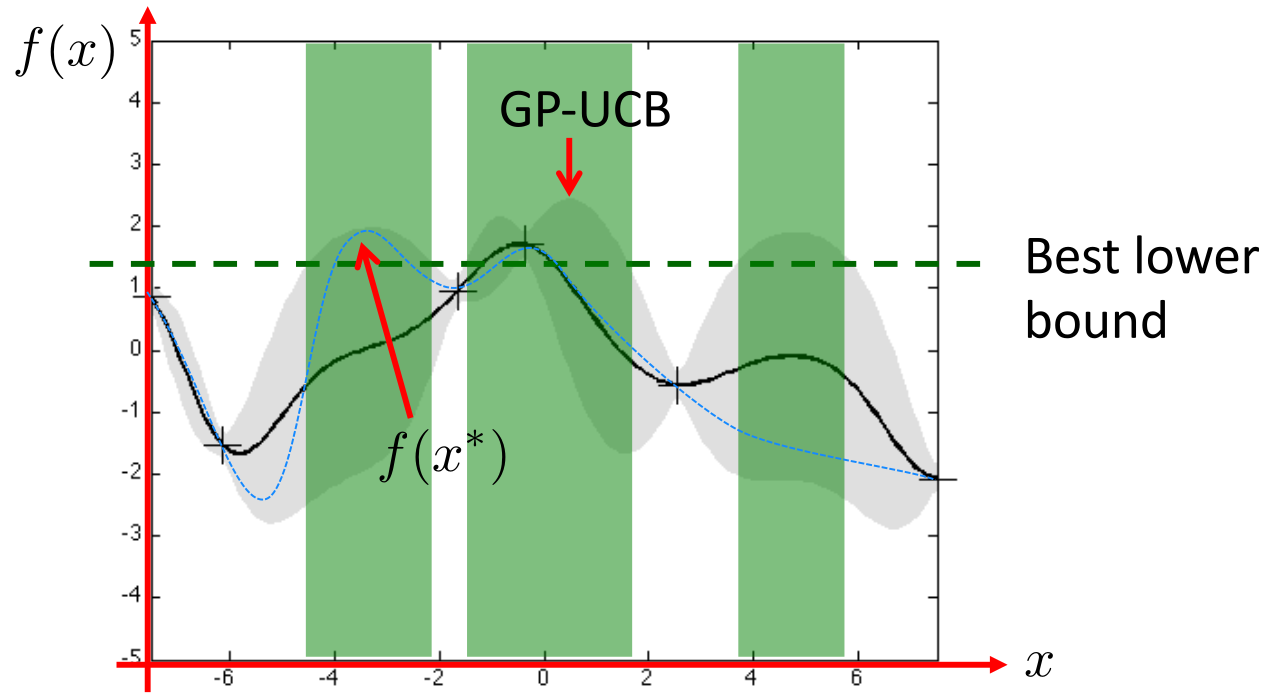
\includegraphics[width=1.0\textwidth]{src/bayesian_optimization/figures/gp-ucb.png}
  \end{figure}
  This idea can be utilized in various ways:
  \begin{itemizenosep}
    \item GP-UCB \cref{subsubsec:gaussian_process-ucb}
    \item Thompson Sampling \cref{subsubsec:thompson_sampling}
  \end{itemizenosep}
\end{sectionbox}
%%% Local Variables:
%%% mode: latex
%%% TeX-command-extra-options: "-shell-escape"
%%% TeX-master: "../../../formulary"
%%% End:

      \subsubsection{Gaussian Process-UCB}\label{subsubsec:gaussian_process-ucb}
        \begin{principbox}\nospacing
  \begin{princip}[Optimization in the phase of uncertainty]\label{princip:optimization_in_the_phase_of_uncertainty}
    Pick the action that has the highest upper confidence bound (UCP).
  \end{princip}
\end{principbox}
\begin{explanationbox}
  \begin{explanation}[\cref{princip:optimization_in_the_phase_of_uncertainty}]
    We do not pick the action that maximizes our current estimate $\mean(x)$ but
    the most optimistic one.\\
    If the guess is wrong optimism will fade quickly but if the guess is right
    we will maximize our utility will decreasing uncertainty.
  \end{explanation}
\end{explanationbox}
\begin{defnbox}\nospacing
  \begin{defn}[GP-UCB]\label{defn:gp-ucb}
    \begin{align}
      \xvec_{t}=\argmax_{x\in D}\mean_{t-1}(\xvec)+\betac_{t}\std_{t-1}(\xvec)
    \end{align}
  \end{defn}
\end{defnbox}
\begin{explanationbox}
  \begin{explanation}[Definition~\ref{defn:gp-ucb}]\leavevmode
    \begin{itemizenosep}
      \item $\betac_{t}\to\infty$ recover uncertainty sampling
      \item $\betac_{t}=0$ recover greedy algorithm
    \end{itemizenosep}
  \end{explanation}
\end{explanationbox}
\subsubsubsection{Maximizing the UCB}\label{subsubsubsec:maximizing_the_ucb}
\begin{sectionbox}\nospacing
  The GP-UCB\cref{defn:gp-ucb} is usually a non-convex function. Thus in order to maximize this objective
  we need to use:
  \begin{itemizenosep}
    \item \textit{Lipschitz Optimization} (in low dimension)
    \item Use gradient descent based on multiple random initialization (in high dimension)
  \end{itemizenosep}
\end{sectionbox}
\subsubsubsection{Guarantees on the regret}\label{subsubsubsec:guarantees_on_the_regret}
\begin{theorembox}\nospacing
  \begin{theorem}[Bayesian Regret of GP-UCB]\label{theorem:bayesian_regret_of_gp-ucb}
    assuming the true function $f$ follows a Gaussian Process $f\distas\GP$ then it holds that
    for a suitable choice of $\betac_{t}$ (needs to slowly decay with const$\cdot\log t$):
    \begin{align*}
      \frac{1}{T}\sum_{t=1}^{T}\left[f(\xvec^*)-f(\xvec_{t})\right]=\bigO \left(\frac{\gammac_{T}}{T}\right)&&T:\text{ \#of samples}
    \end{align*}
    with\hfil$\gammac_{T}=\max_{\abs{S}\leq T}I(f;y_{S})$
  \end{theorem}
\end{theorembox}
\begin{explanationbox}
  \begin{explanation}[$\gammac_{T}$]
    The regret depends on how much information we can gain in $T$ steps.
  \end{explanation}
\end{explanationbox}
\begin{corbox}\nospacing
  \begin{cor}[Linear Kernel]\leavevmode\\
    For a linear kernel\cref{defn:linear_kernel} it holds:
    \begin{align}
      \gammac_{T}=\bigO(d\log T)
    \end{align}
  \end{cor}
\end{corbox}
\begin{corbox}\nospacing
  \begin{cor}[Squared Exponential Kernel]\leavevmode\\
    For a squared exponential kernel\cref{defn:ml_gaussian_rbf_squared_exponential_kernel} it holds:
    \begin{align}
      \gammac_{T}=\bigO*{(\log T)^{d+1}}
    \end{align}
  \end{cor}
\end{corbox}
\begin{corbox}\nospacing
  \begin{cor}[Matern Kernel $\nuc>2$]\leavevmode\\
    For a linear kernel\cref{defn:ml_matern_kernel} it holds:
    \begin{align}
      \gammac_{T}=\bigO*{T^{\frac{d(d+1)}{2\nuc+d(d+1)}}}
    \end{align}
  \end{cor}
\end{corbox}
\begin{notebox}[Note: Reproducing Kernel Hilbert Space (RKHS)]\nospacing
  There exists also a frequentists regret of GP-UCB which only assumes that $f$ is part of a hilbert space
  and overinflates the confidence bounds in order to obtain good estimates.
\end{notebox}
%%% TeX-command-extra-options: "-shell-escape"
%%% Local Variables:
%%% mode: latex
%%% TeX-master: "../../../formulary"
%%% End:

      \subsubsection{Thompson Sampling}\label{subsubsec:thompson_sampling}
        \begin{defnbox}\nospacing
  \begin{defn}[Thompson Sampling]\label{defn:thompson_sampling}
    Draw a function $\widetilde{f}$ from the posterior and maximize it:
    \begin{align}
      \widetilde{f}\distas\prob(f|\xvec_{1:n},\yvec_{1:t})&&\xvec_{t+1}\in\argmax_{\xvec\in D}\widetilde{f}(\xvec)
    \end{align}
  \end{defn}
\end{defnbox}
\begin{explanationbox}
  \begin{explanation}[Definition~\ref{defn:thompson_sampling}]
    The randomness in $\widetilde{f}$ helps to trade of exploration vs.\ exploitation.
  \end{explanation}
\end{explanationbox}
%%% Local Variables:
%%% mode: latex
%%% TeX-master: "../../../formulary"
%%% TeX-command-extra-options: "-shell-escape"
%%% End:










% ------------------------------------------------------------------------------ 
% ======================================================================
% TODO
% ======================================================================
% \input{src/General_TODO.tex}
% \newpage
\section*{Machine Learning Appendix}\label{sec:ml_appendix}
  \input{ml_submodule/ml.tex}
\newpage
\section*{Math Appendix}\label{sec:math_appendix}
\input{math_submodule/math.tex}
% ==============================================================================
% Document end
% ==============================================================================
\end{document}




%%% Local Variables:
%%% mode: latex
%%% TeX-command-extra-options: "-shell-escape"
%%% TeX-master: t
%%% End:
